\documentclass[../Main/Knit.tex]{subfiles}
\newpage

\section{Iso-Seq: Optimisation} 

ERCC was used to assess the sensitivity and quality of whole transcriptome Iso-Seq runs and to optimise the bioinformatics pipeline (Figure X) by determining the number of ERCCs detected after:
\begin{enumerate}
	\item varying the CCS parameters, which would affect the number of FL reads post Iso-Seq cluster
	\item varying any additional parameters in cupcake collapse and usage of additional tools for filtering
\end{enumerate}

\subsection{Varying CCS parameters}
As described in Section \ref{section:classify}, the proportion of raw subreads that can be successfully collapsed to generate a CCS is widely influenced by the number of passes (default: 3 passes) and minimum base accuracy (default: 99\%), which settings are widely varied in scientific community. 

To determine the most optimum parameters for CCS generation, CCS was generated on a subset of 1 sample using a combination of parameters, and then further validated with 2 whole samples (Figure \ref{fig:ccs_optimisation}):
\begin{figure}[h!]
	\centering
	\begin{subfigure}{0.8\linewidth}
		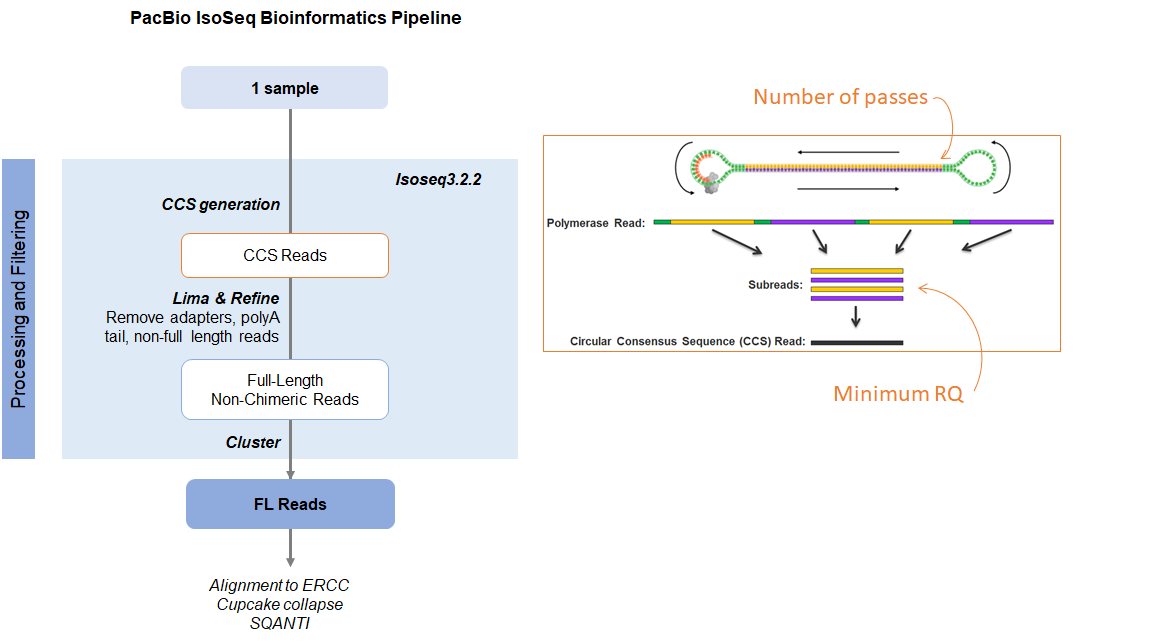
\includegraphics[width=\linewidth, height=0.3\textheight]{../Pictures/ERCC_Pipeline.png}
		\caption{Factors influencing successful CCS generation of raw subreads}
	\end{subfigure}
	\hspace{2em}
	\begin{subfigure}{0.4\linewidth}
		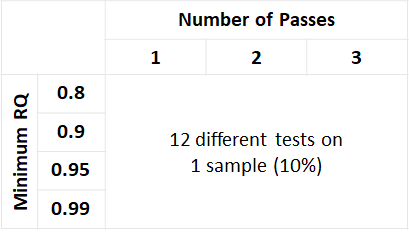
\includegraphics[width=\linewidth, height=0.12\textheight]{../Pictures/ERCC_firstoptim.png}
		\caption{1st CCS parameter optimisation}
	\end{subfigure}
	\hspace{2em}
	\begin{subfigure}{0.4\linewidth}
		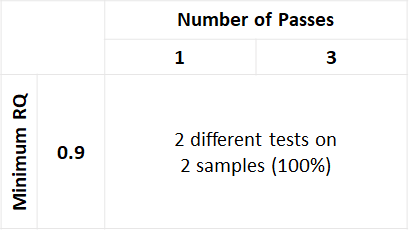
\includegraphics[width=\linewidth, height=0.12\textheight]{../Pictures/ERCC_secondoptim.png}
		\caption{2nd CCS parameter optimisation}
	\end{subfigure}
	\captionsetup{width=0.95\textwidth}
	\caption[Optimisation of CCS generation]%
	{\textbf{Optimisation of CCS generation}: Successful CCS generation of raw subreads is dependent on the number of polymerase passes and minimum RQ of subreads. A two-step approach was taken to determine the optimum parameters, using (b) whole range of parameters on 10\% of one sample, and (c) extending analyses to two samples but with a more refined combination (as determined from the results of first step))}
	\label{fig:ccs_optimisation}
\end{figure} 


Conclusion: 0.9 and 1 pass 

- Results of number of reads and ERCCs detected (first and second round)

\newpage
\subsection{Additional parameters}

To assess the sensitivity across Iso-Seq runs to detect ERCC, a merged analysis of whole transcriptome samples (n = 10, WT = 5, TG = 5) was performed with ERCC alignment and further collapse using Cupcake. The counts of full-length transcripts pertaining to each sample were then obtained using a custom demultiplexed script, which classifies and counts the merged data based on the unique sequencing run id. Post SQANTI annotation and filtering, only a third of ERCCs (unique number of ERCC = 37, 40.22\%) were identified from both WT (mean number of ERCC: 32.4 (35\%)) and TG (mean number of ERCC: 32.2 (35.22\%)), with no difference in number of ERCC detected between WT and TG, although there were some ERCC that were detected in WT but not in TG, and vice versa. A minority of ERCCs (n = 8, 8.7\%) at higher concentration were further annotated with more than one "isoform", indicating the presence of technical artefacts and more stringent filtering or clustering required, with ERCC at a higher concentration more likely to be sequenced and annotated with multiple redundant "isoforms". Exploration of these "isoforms" revealed them to be shorter transcripts likely to be generated as a result of fragmentation of the original molecule, incomplete PCR synthesis and template-switching. Application of TAMA-GO's script, tama-remove-fragment-models.py, successfully removed these partial, redundant isoforms, while retaining the intact isoforms. 

Deeper investigation into the low coverage of ERCCs further identified an additional 20 lowly-expressed ERCCs that were discarded from cupcake's collapse scripts under the default coverage (alignment identity) parameters at 99\%. Exploration of these imperfect-aligned sequences revealed 5'prime degradation of XX-XX nucleotides - one of the limitations of not using a 5'cap protocol. Inclusion of these ERCCs using a lower minimum coverage threshold at 95\% increased the number of ERCCs detected by 20\% (unique number of ERCC = 57, 61.96\%), and strengthening the relationship between full-length read count and known amount of ERCC (95\% coverage: corr = 0.98, p = 1.41 x 10\textsuperscript{-41}; 99\% coverage: corr = 0.82, p = 4.89 x 10\textsuperscript{-10}).   

Several learnings were taken from analysis with ERCC: i) default parameters used in cupcake collapse, particularly alignment identity, are too stringent with removal of true transcripts, and ii) need for additional filtering using TAMA-GO's scripts to remove partial transcripts.

- Pipeline figure 
- a) unique ERCC b) isoform vs con, correlation
- a) tama removal, b) tama removal further 
- a) mapping 
- a) readjustment, unique ERCC, lowly expressed transcipts, correlation

\begin{figure}[h]
	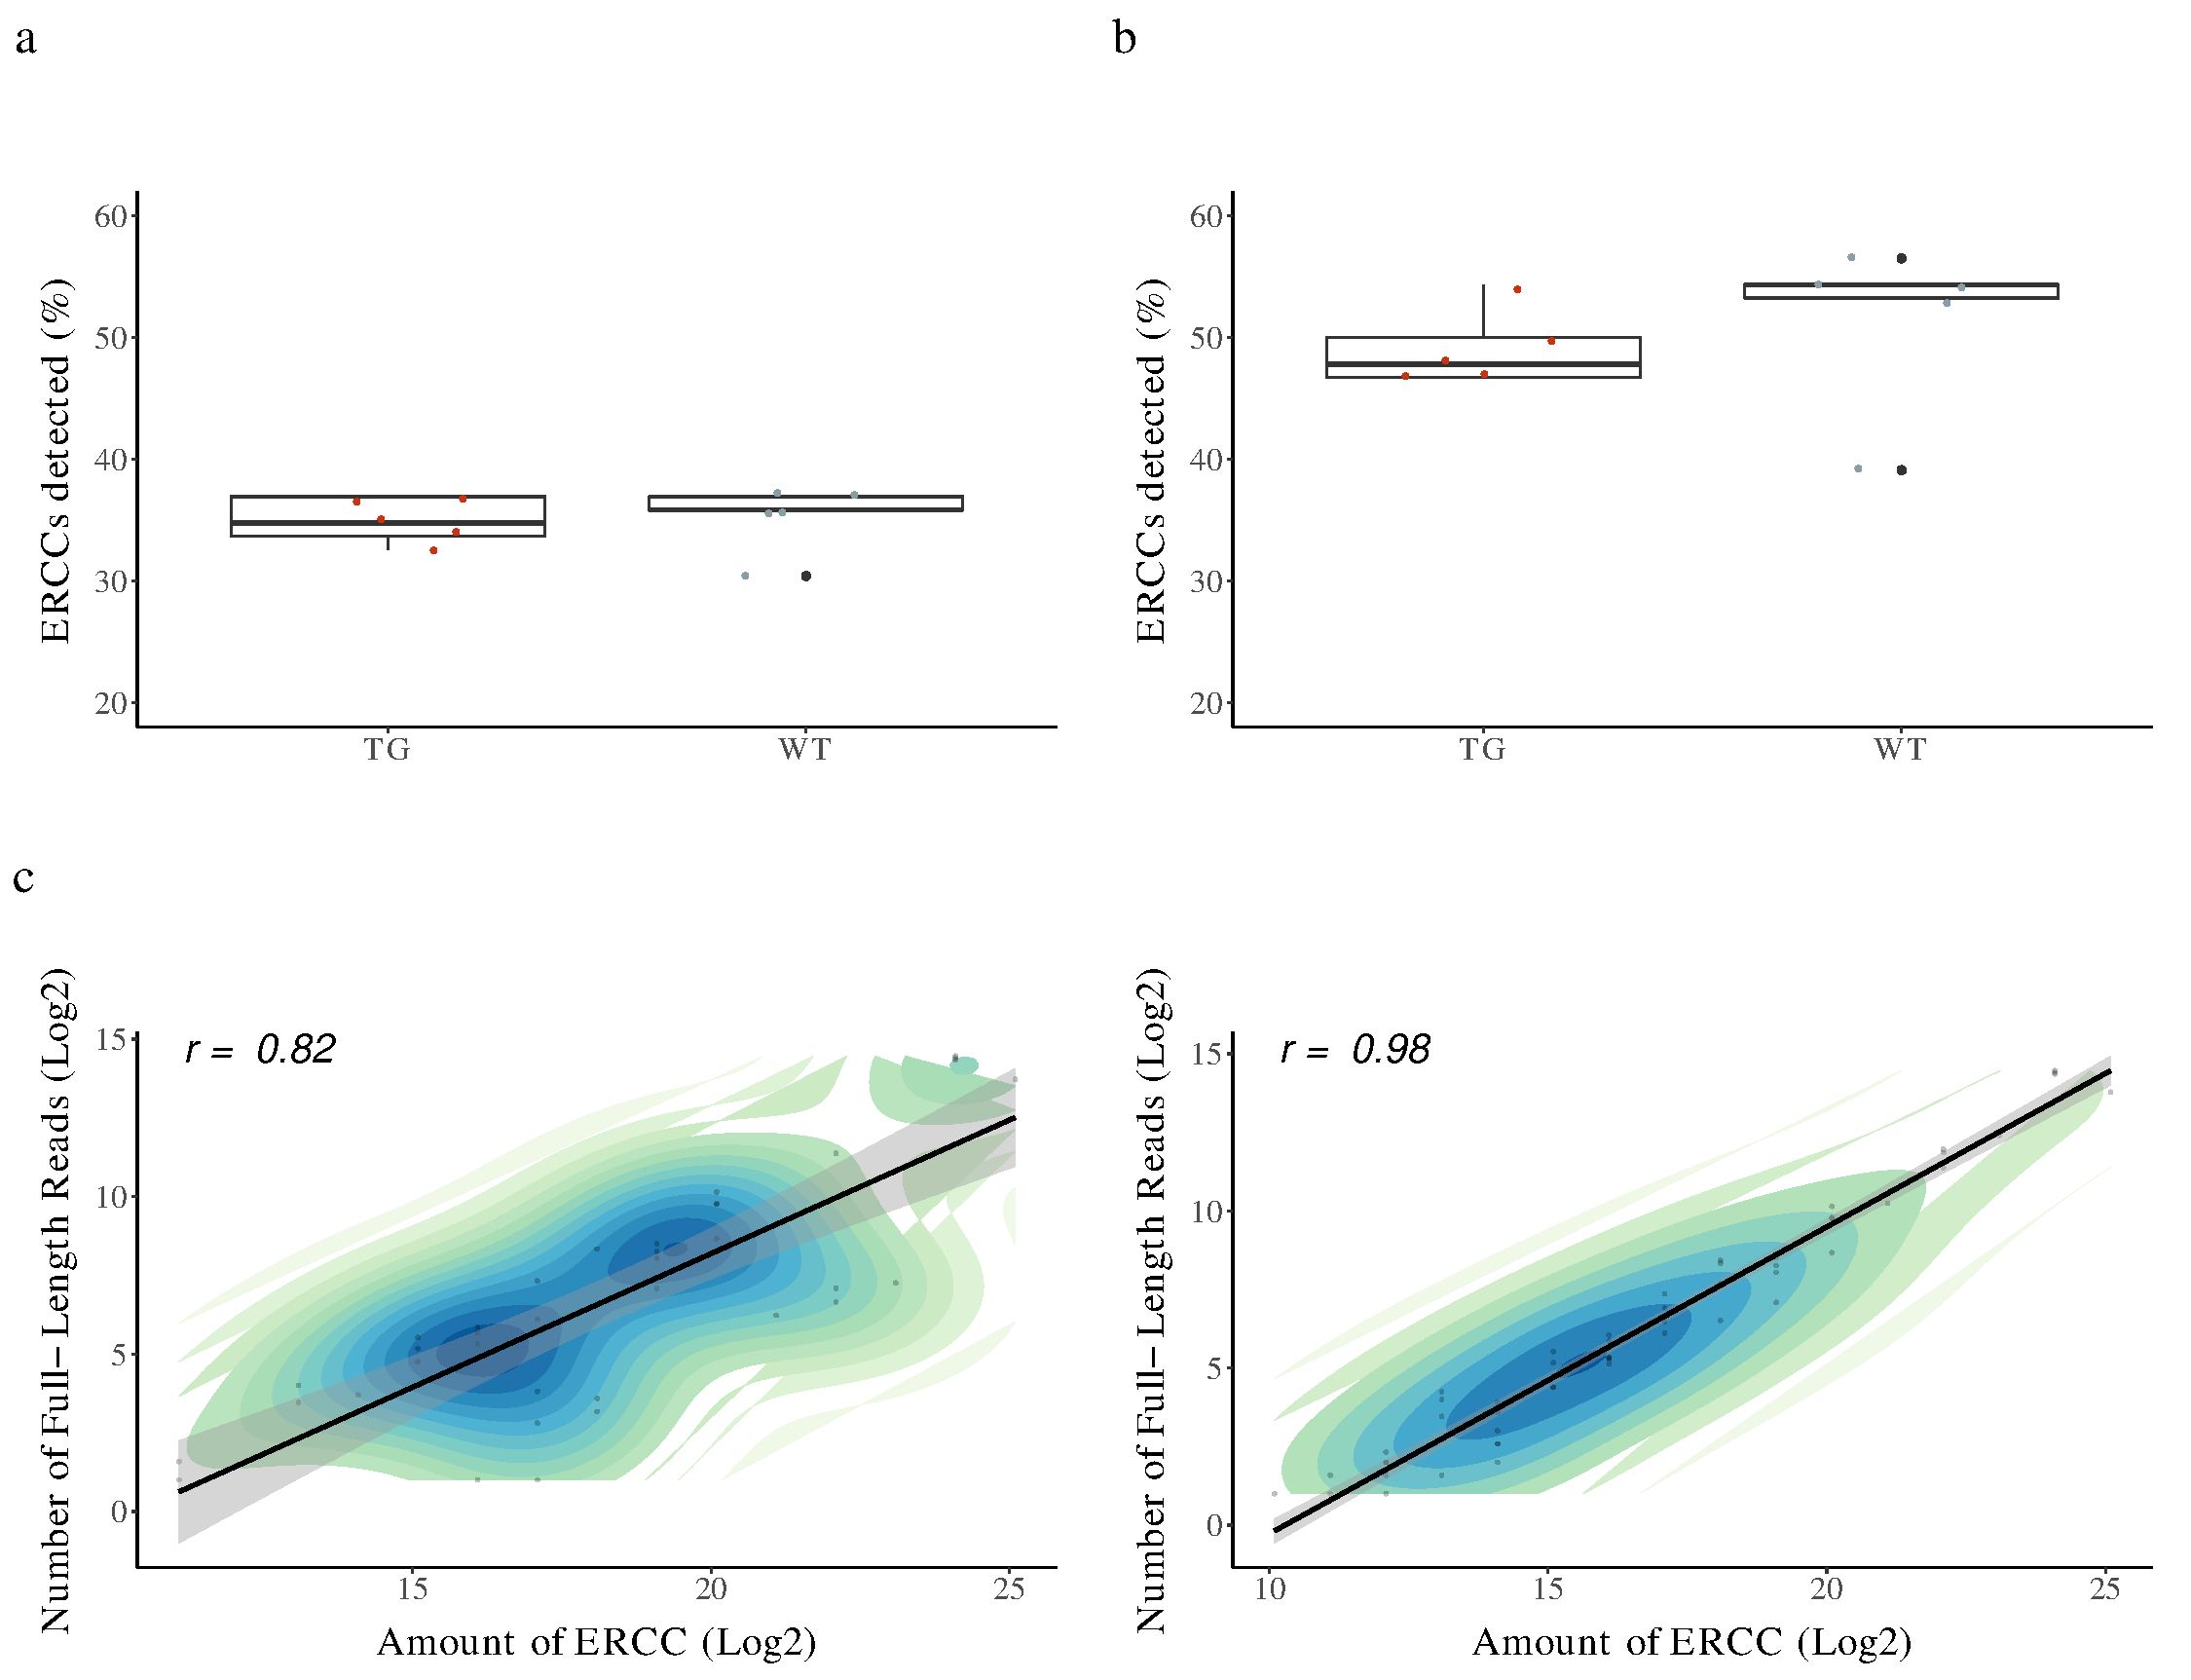
\includegraphics[page=1, width=1\linewidth,height=0.4\textheight]{../Pictures/Project_Development/ERCC.pdf}
	\captionsetup{width=0.95\textwidth}
	\caption[No significant correlation between RIN and Whole Transcriptome Iso-Seq run output]%
	{\textbf{No significant correlation between RIN and Whole Transcriptome Iso-Seq run output}: Samples with RIN $>$8 were selected for Whole Transcriptome Iso-Seq, with TG samples having distinctly lower RIN values than WT samples. However, no significant difference was observed for run output between WT and TG (Figure \ref{tab:run_output}) }
	\label{fig:uniqueERCC}
\end{figure}

\begin{figure}[h]
	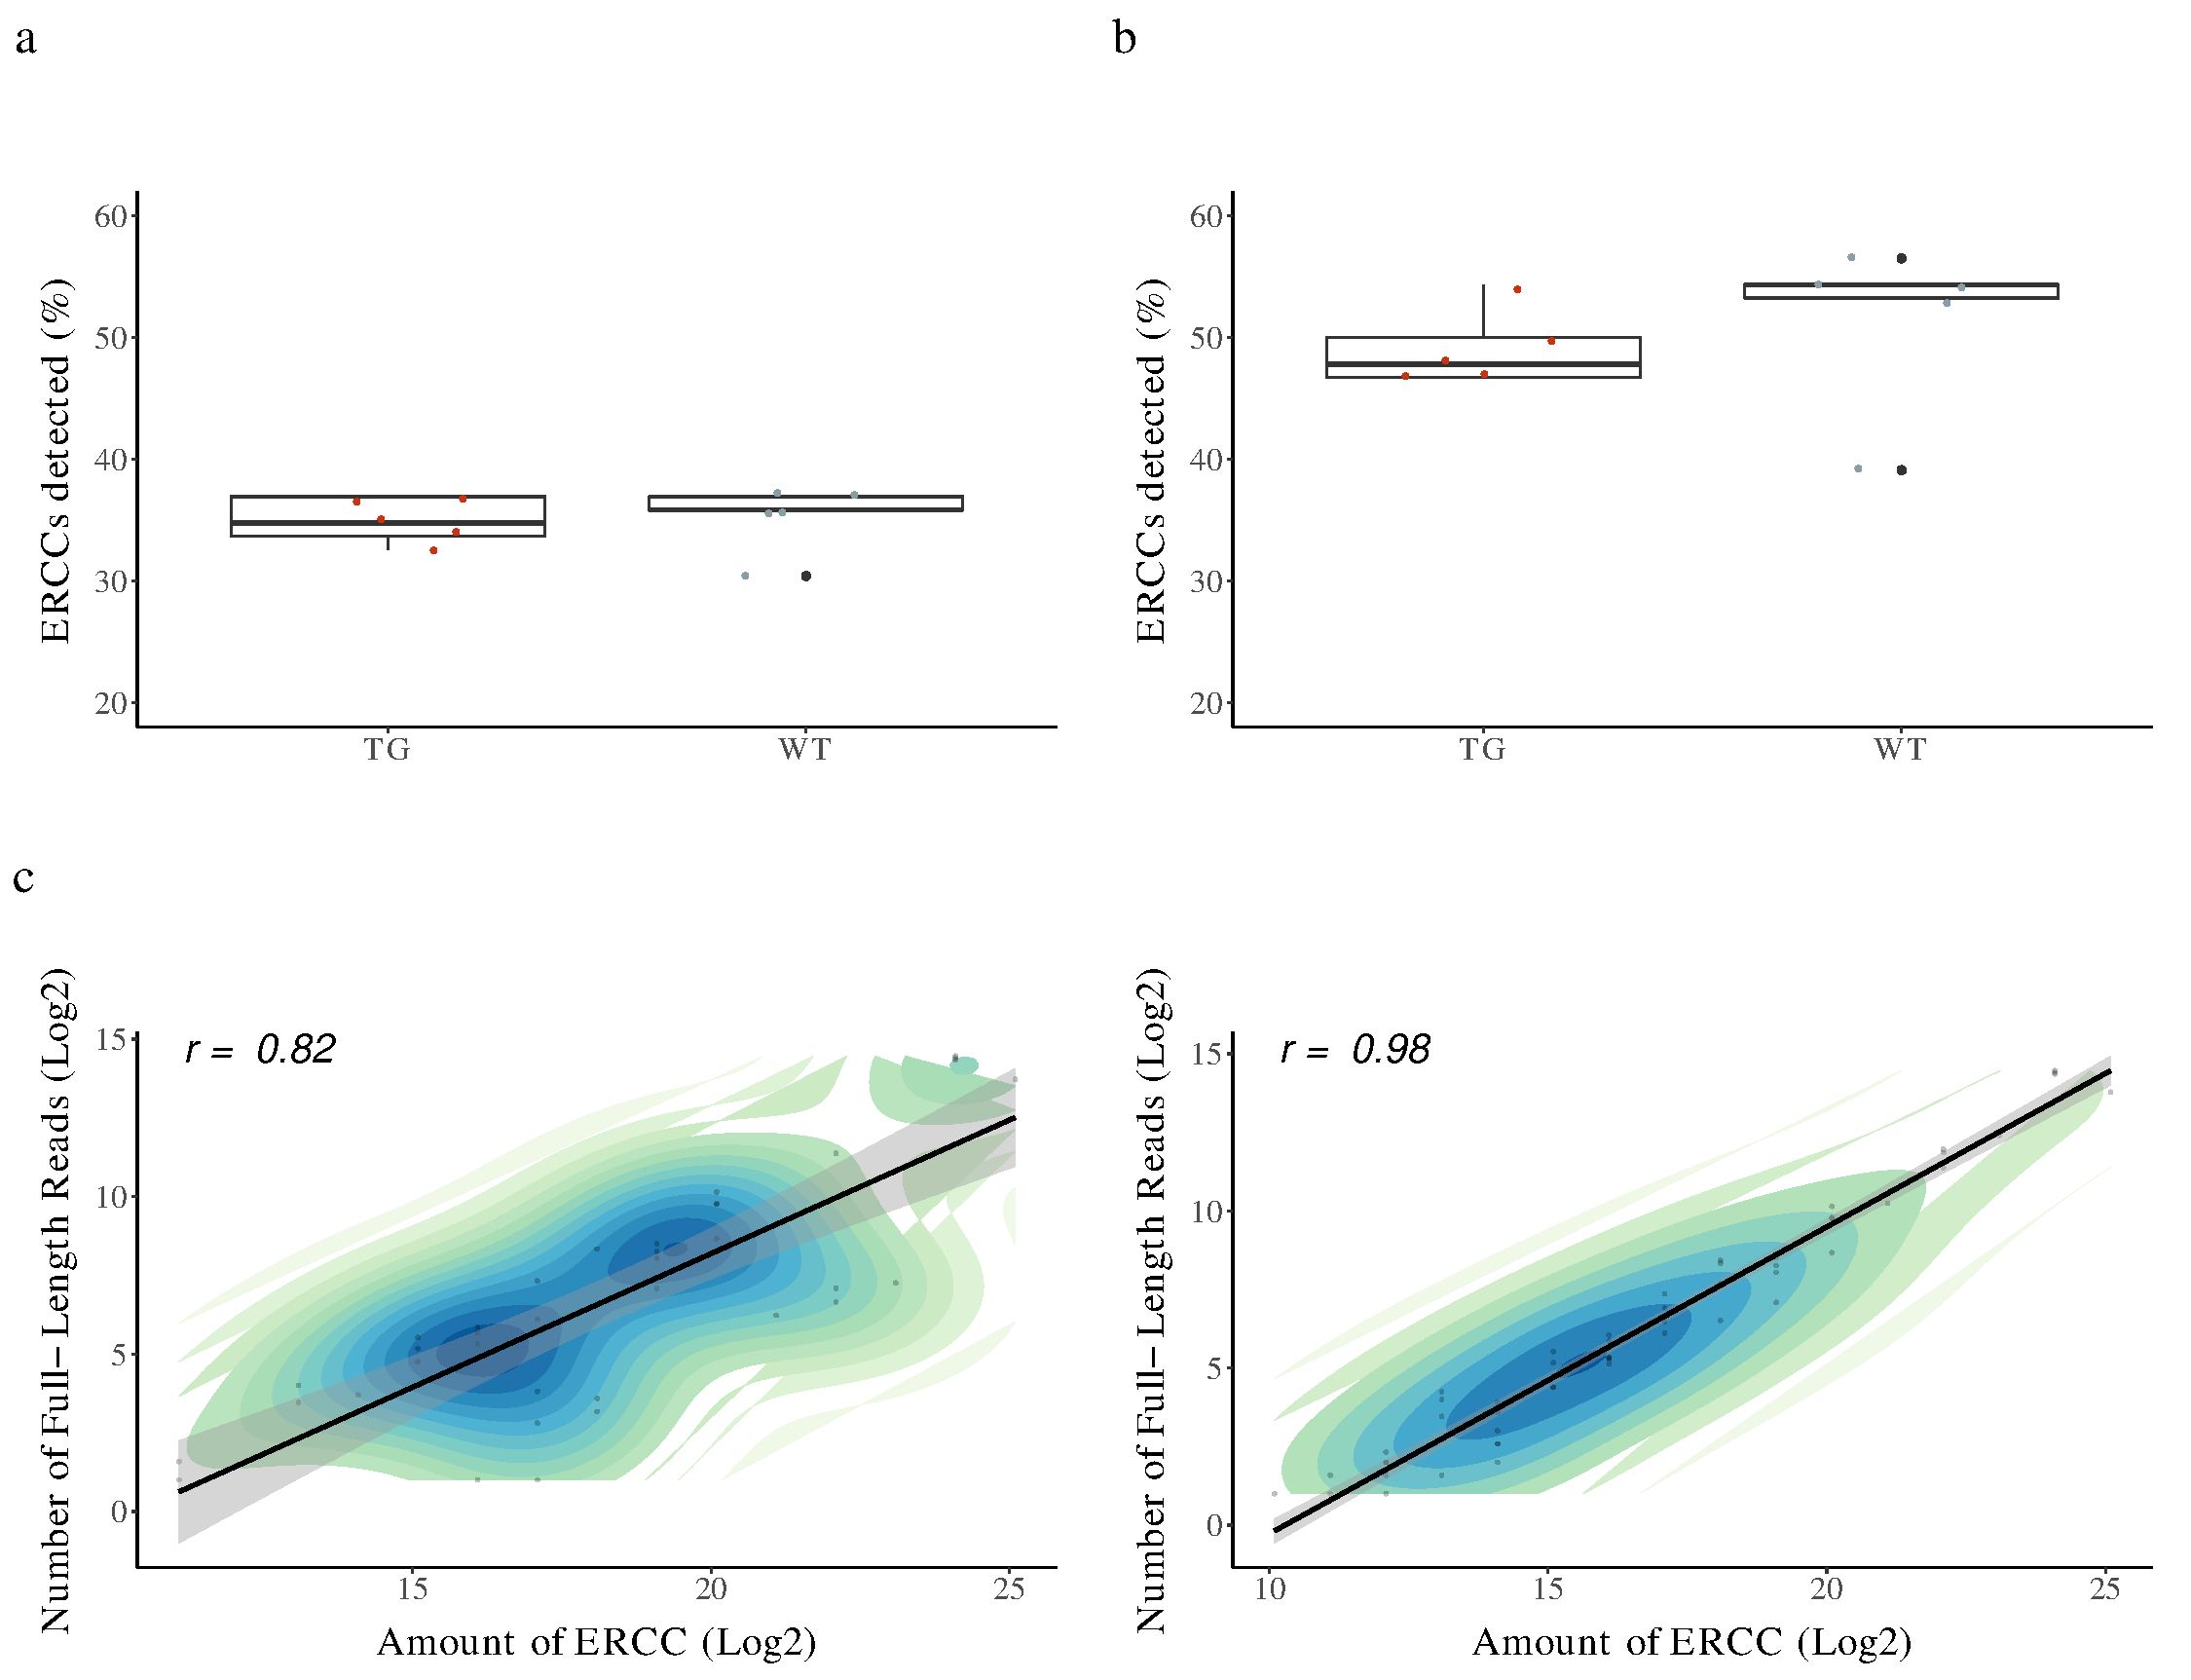
\includegraphics[page=1, width=1\linewidth,height=0.4\textheight]{../Pictures/Project_Development/ERCC.pdf}
	\captionsetup{width=0.95\textwidth}
	\caption[No significant correlation between RIN and Whole Transcriptome Iso-Seq run output]%
	{\textbf{No significant correlation between RIN and Whole Transcriptome Iso-Seq run output}: Samples with RIN $>$8 were selected for Whole Transcriptome Iso-Seq, with TG samples having distinctly lower RIN values than WT samples. However, no significant difference was observed for run output between WT and TG (Figure \ref{tab:run_output}) }
	\label{fig:uniqueERCC}
\end{figure}
 
\subsubsection{Application of additional parameters to Whole Transcriptome}
A merged analysis of whole transcriptome samples (n = 12, WT = 6, TG = 6) was performed with alignment to the mouse genome (mm10), with 276,035 reads (99.3\%) mapped to mouse genome, 365 reads (0.13\%) mapped to ERCC and 1,568 reads (0.56\%) unmapped. 

 using cupcake's collapse default (99\%) and reduced threshold (85\%) for alignment identity. 
